\section{Layout of Presentation Markup}

\subsection{Token Elements}

...

\subsection{General Layout Schemata}

\subsubsection{Horizontally Group Sub-Expressions {\tt <mrow>}}

...

\subsubsection{Fractions {\tt <mfrac>}}

The {\tt mfrac} element is used for fractions. It can also be used to mark up
fraction-like objects such as binomial coefficients and Legendre symbols.
The syntax for {\tt mfrac} is

\begin{lstlisting}
  <mfrac> numerator denominator </mfrac>
\end{lstlisting}

The {\tt mfrac} element sets {\tt displaystyle} to "false", or if it was
already false increments scriptlevel by 1, within numerator and denominator.
This can be achieved with the following style in the user agent stylesheet:

\begin{lstlisting}
  mfrac > * {
    mathml-script-level: auto;
    mathml-math-style: inline;
  }
\end{lstlisting}

The default line thickness is given by {\tt FractionRuleThickness}
Use the {\tt linethickness} attribute \cite{MathML3} to determine the
actual thickness of the fraction bar. A percent or unitless length is
interpreted as a multiple of the default rule thickness and
the named values "thin", "medium" and "thick" are interpreted as
50\%, 100\%, 200\%.
The color and visibility of the fraction bar must honor the values given by the
{\tt color} and {\tt visibility} CSS properties.

If the actual linethickness is nonzero, the {\tt mfrac} element is laid out as
shown on \ref{FractionBoxModel}. The width is given by the maximum width of the
numerator and denominator and the numerator and denominator are horizontally
centered. A fraction bar with the actual thickness is drawn centered on the
axis height. The numerator and denominator are shifted
up and down using the values {\tt FractionNumeratorShiftUp},
{\tt FractionDenominatorShiftDown} in inline style and
{\tt FractionNumeratorDisplayStyleShiftUp},
{\tt FractionDenominatorDisplayStyleShiftDown} in display style.
If necessary, these shift values are increased to ensure that the gaps between
the numerator/denominator and fraction bar satisfy the minimal values provided
by {\tt FractionDenominatorGapMin} and
{\tt FractionNumeratorGapMin} in inline style and
{\tt FractionDenominatorDisplayStyleGapMin} and
{\tt FractionNumeratorDisplayStyleGapMin} in display style.

\begin{figure}
\centering
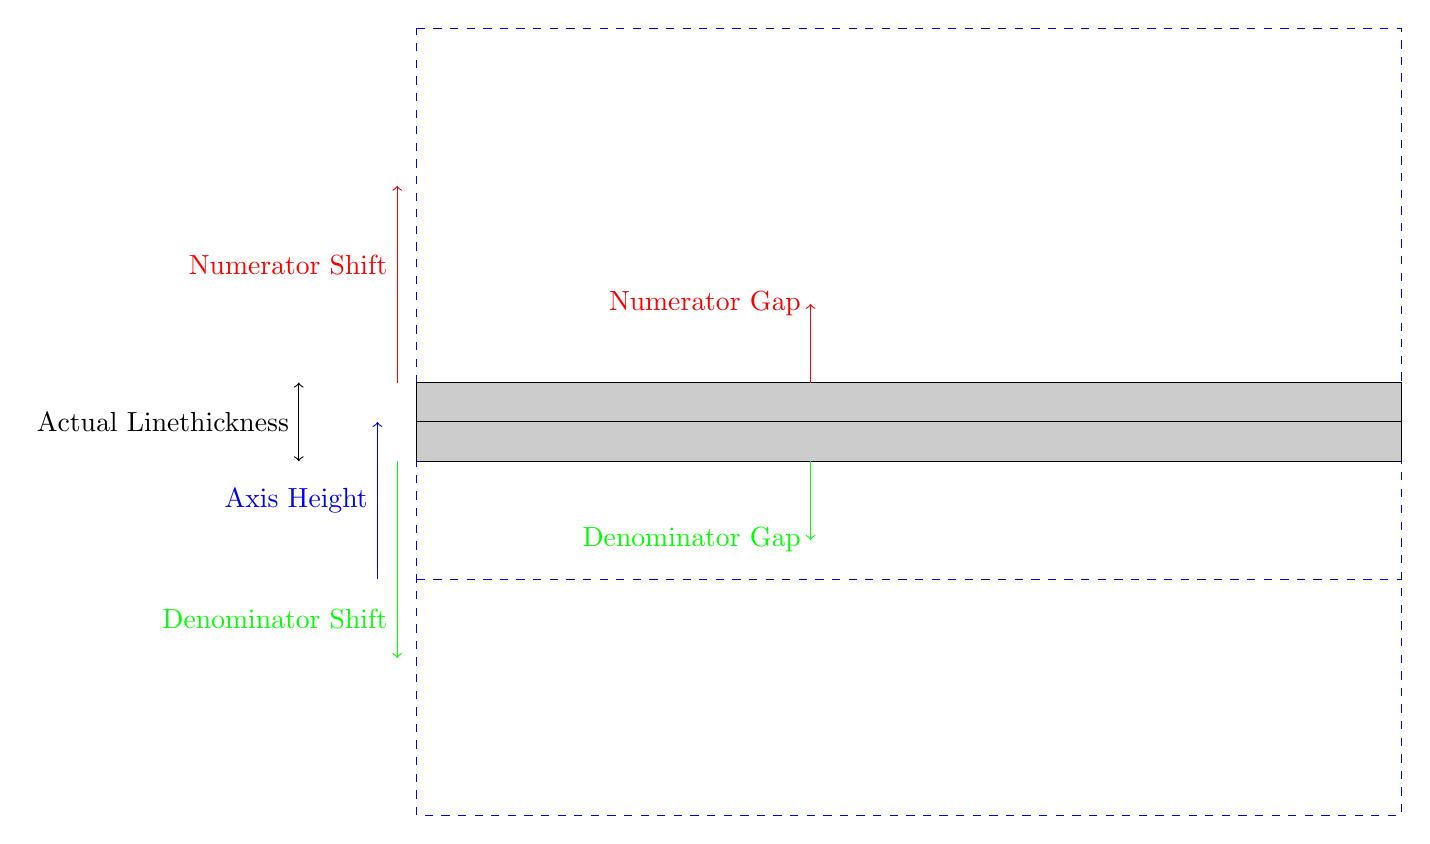
\begin{tikzpicture}[yscale=-1]
  \MathMLBox{0}{-5}{2.5}{1}{red}
  \MathMLBox{3.75}{1}{1}{1}{green}
  \draw[dashed,blue] (0,-7) -- (12.5,-7) -- (12.5,3) -- (0,3) -- cycle
  (0,0) -- (12.5,0);
  \fill[black!20] (0,-2.5) -- (12.5,-2.5) -- (12.5,-1.5) -- (0,-1.5) -- cycle;
  \draw[black] (0,-2.5) -- (12.5,-2.5) -- (12.5,-1.5) -- (0,-1.5) -- cycle
  (0,-2) -- (12.5,-2);
  \draw[->,blue] (-.5,0) -- (-.5,-1) node[left]{Axis Height} -- (-.5,-2);
  \draw[<->,black] (-1.5,-2.5) --
  (-1.5,-2) node[left]{Actual Linethickness} -- (-1.5,-1.5);
  \draw[->,red] (-.25,-2.5) -- (-.25,-4)
  node[left]{Numerator Shift} -- (-.25,-5);
  \draw[->,green] (-.25,-1.5) -- (-.25,.5)
  node[left]{Denominator Shift} -- (-.25,1);
  \draw[->,red] (5,-2.5) -- (5,-3.5) node[left]{Numerator Gap};
  \draw[->,green] (5,-1.5) -- (5,-.5) node[left]{Denominator Gap};
\end{tikzpicture}
\label{FractionBoxModel}
\end{figure}

If the actual linethickness zero, the {\tt mfrac} element is instead laid out as
shown on \ref{StackBoxModel}. The relevant shift values are now
{\tt StackTopShiftUp},
{\tt StackBottomShiftDown} in inline style and
{\tt StackTopDisplayStyleShiftUp},
{\tt StackBottomDisplayStyleShiftDown} in display style.
If necessary, the two shift values are increased by a same value to ensure
the gaps between the top and bottom boxes satisfy the values provided by
by {\tt StackGapMin} in inline style and
{\tt StackDisplayStyleGapMin} in display style.

\begin{figure}
\centering
\begin{tikzpicture}[yscale=-1]
  \MathMLBox{0}{-5}{2.5}{1}{red}
  \MathMLBox{3.75}{1}{1}{1}{green}
  \draw[dashed,blue] (0,-7) -- (12.5,-7) -- (12.5,3) -- (0,3) -- cycle
  (0,0) -- (12.5,0);
  \draw[black,dashed] (0,-2) -- (12.5,-2);
  \draw[->,blue] (-.5,0) -- (-.5,-1) node[left]{Axis Height} -- (-.5,-2);
  \draw[->,red] (-.25,-2) -- (-.25,-4)
  node[left]{Stack Top Shift} -- (-.25,-5);
  \draw[->,green] (-.25,-2) -- (-.25,.5)
  node[left]{Stack Bottom Shift} -- (-.25,1);
  \draw[<->,blue] (5,-3.5) -- (5,-1.5) node[left]{Stack Gap} --
  (5,-.5);
\end{tikzpicture}
\label{StackBoxModel}
\end{figure}

User agents may increase the width by adding a trailing/leading space
of 1 pixel around the fraction. If the numerator is an embellished operator and
the {\tt mfrac} element is the outermost element in this embellished operator
hierarchy then the operator leading and trailing spaces must be added around
the fraction.

User agents may extend the box model to support the {\tt numalign},
{\tt denomalign} and {\tt bevelled} attributes \cite{MathML3}.

\subsubsection{Radicals {\tt <msqrt>}, {\tt <mroot>}}

These elements construct radicals. The {\tt msqrt} element is used for square
roots, while the {\tt mroot} element is used to draw radicals with indices,
e.g. a cube root. The syntax for these elements is:

\begin{lstlisting}
  <msqrt> base </msqrt>
  <mroot> base index </mroot>
\end{lstlisting}

The {\tt mroot} element requires exactly 2 arguments. However, {\tt msqrt}
accepts a single argument, possibly being an inferred {\tt mrow} of multiple
children.

The {\tt mroot} element increments scriptlevel by 2, and sets displaystyle to
"false", within index, but leaves both attributes unchanged within base. The
{\tt msqrt} element leaves both attributes unchanged within its argument.
This can be achieved with the following style in the user agent stylesheet:

\begin{lstlisting}
  mroot > :not(:first-child) {
    mathml-script-level: +2;
    mathml-math-style: inline;
  }
\end{lstlisting}

The line thickness of the overbar is given by {\tt RadicalRuleThickness}.
The gap between the overbar and base is given by {\tt RadicalVerticalGap}
in inline style and {\tt RadicalDisplayStyleVerticalGap} in display style.
The ascent above the overbase is given by {\tt RadicalExtraAscender}. The
surd is drawn by trying to vertically stretch the character U+221A SQUARE ROOT
to at least the sum of the ink height of the base, the radical gap and the
radical rule thickness. If the CSS {\tt direction} is set to right-to-left,
then the surd is actually drawn from the glyph obtained by mirroring
U+221A SQUARE ROOT via the {\tt rtlm} OpenType feature.
The color and visibility of the surd and overbar must honor the values given by
the {\tt color} and {\tt visibility} CSS properties.

The {\tt msqrt} element is laid out as shown on \ref{SquareRootBoxModel}.
The width is given by the sum of the width of the surd and of the base.
The baseline of the square root matches the baseline of the base.
The ink box is determined from the ink boxes of the surd and base while the
logical box takes into account the extra ascender
(add an extra descender ?????).

\begin{figure}
\centering
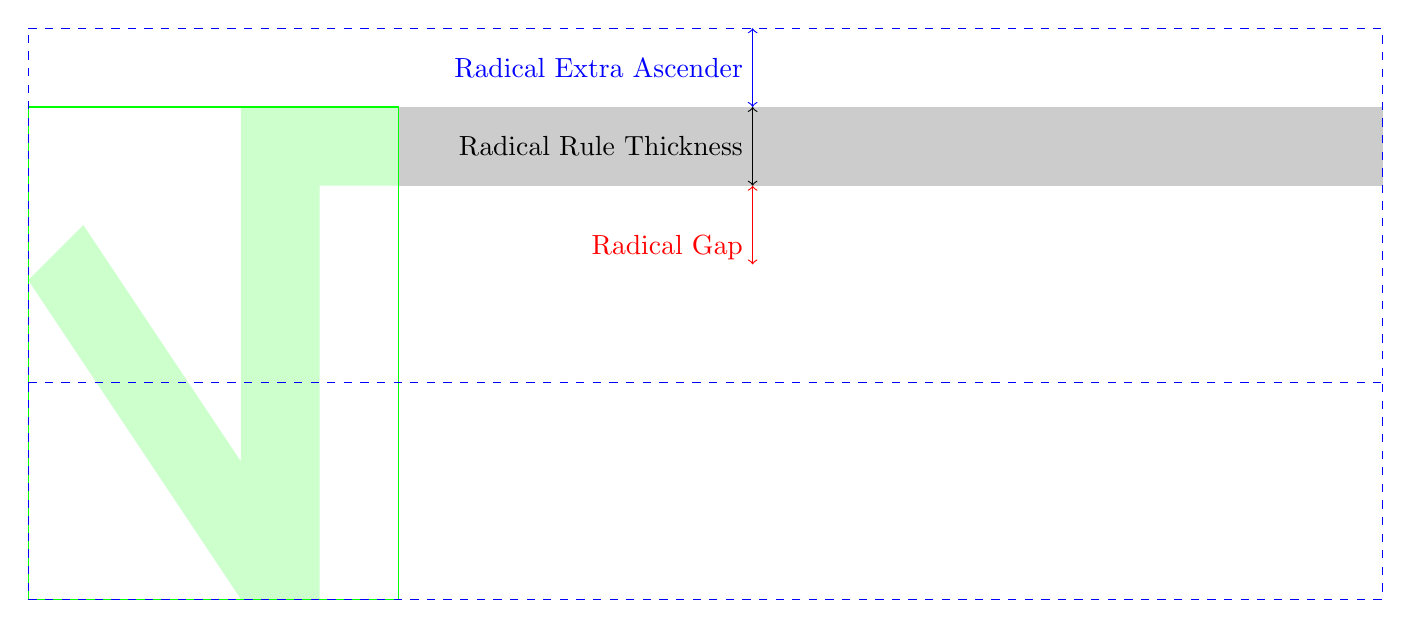
\begin{tikzpicture}[yscale=-1]

  \fill[black!20] (0,-2.5) -- (12.5,-2.5) -- (12.5,-1.5) -- (0,-1.5) -- cycle;

  \fill[green!20]
  (0,-2.5) -- (-2,-2.5) -- (-2,2) --
  (-4,-1) -- (-4.7,-.3) -- (-2.7,2.7) -- (-2,3.75) -- (-1,3.75) --
  (-1,-1.5) -- (0,-1.5) -- (0,-2.5);
  \draw[green] (-4.7,-2.5) -- (0,-2.5) -- (0,3.75) -- (-4.7,3.75) -- cycle;

  \MathMLBox{0}{1}{2.5}{1}{red}

  \draw[dashed,blue] (-4.7,-3.5) -- (12.5,-3.5) --
                     (12.5,3.75) -- (-4.7,3.75) -- cycle
                      (-4.7,1) -- (12.5,1);

  \draw[<->,blue] (4.5,-3.5) --
  (4.5,-3) node[left]{Radical Extra Ascender} -- (4.5,-2.5);

  \draw[<->,black] (4.5,-2.5) --
  (4.5,-2) node[left]{Radical Rule Thickness} -- (4.5,-1.5);

  \draw[<->,red] (4.5,-1.5) --
  (4.5,-1) node[below left]{Radical Gap} -- (4.5,-.5);
\end{tikzpicture}
\label{SquareRootBoxModel}
\end{figure}

The {\tt mroot} element is laid out as shown on \ref{RootBoxModel}.
We start by ignoring the root index and we layout the base and surd as
shown on \ref{SquareRootBoxModel} to obtain a box $B$.
The horizontal metrics of the {\tt mroot} element are obtained by putting
{\tt RadicalKernBeforeDegree}
before the root index, then placing the root index, then a kerning
of {\tt RadicalKernAfterDegree}
after the root index and finally placing $B$ (r. In general
the kerning before the root index is positive while the kerning after it is
negative,
which means that the root element will have some space before it and that the
root index will overlap the surd.
For the vertical metrics of the {\tt mroot} element, we first take the baseline
of $B$ as the baseline. Then if we graduate the ink height of $B$ with a linear
scale going from 0 (bottom) to 1 (top) then the baseline of the root index will
be vertically positioned at coordinate {\tt RadicalDegreeBottomRaisePercent}.
Finally, we take into consideration the box of the root index and $B$ to deduce
the metrics for the whole box of the {\tt mroot} element.

\begin{figure}
\centering
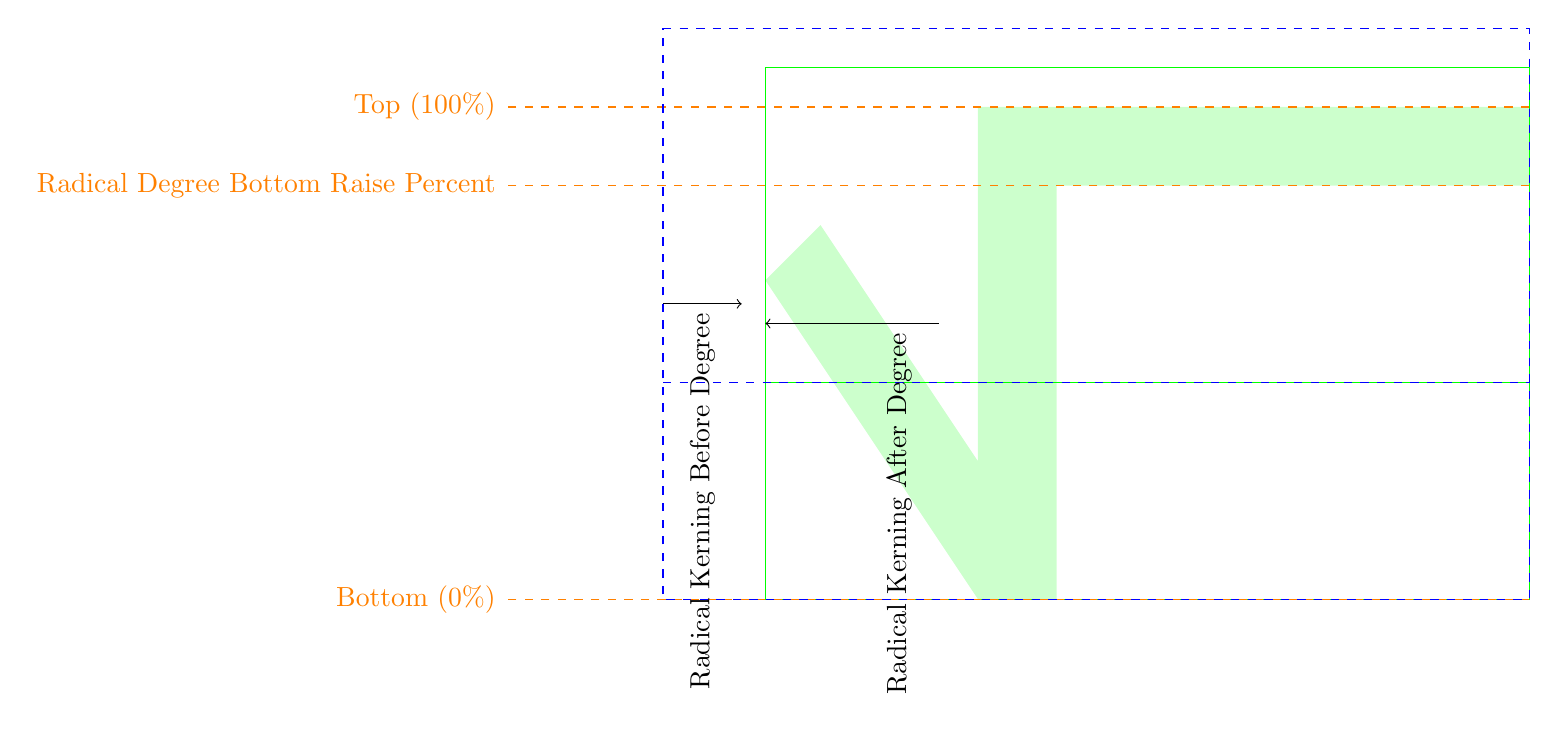
\begin{tikzpicture}[yscale=-1]
  \begin{scope}[shift={(6,0)}]
  \fill[green!20]
  (5,-2.5) -- (-2,-2.5) -- (-2,2) --
  (-4,-1) -- (-4.7,-.3) -- (-2.7,2.7) -- (-2,3.75) -- (-1,3.75) --
  (-1,-1.5) -- (5,-1.5) -- (5,-2.5);
  \draw[green] (-4.7,-3) -- (5,-3) -- (5,3.75) -- (-4.7,3.75) -- cycle
  (-4.7,1)--(5,1);
  \end{scope}

  \MathMLBox{1}{-1.5}{.5}{1}{red}

  \draw[dashed,orange](11,3.75)--(-2,3.75) node[left]{Bottom (0\%)};
  \draw[dashed,orange](11,-1.5)--(-2,-1.5) node[left]{Radical Degree Bottom Raise Percent};
  \draw[dashed,orange](11,-2.5)--(-2,-2.5) node[left]{Top (100\%)};

  \draw[dashed,blue] (0,-3.5) -- (11,-3.5) -- (11,3.75) -- (0,3.75) -- cycle
  (0,1)--(11,1);

  \draw[->,black] (0,0) -- (.5,0) node[left,rotate=90] {Radical Kerning Before Degree} -- (1,0);
  \draw[->,black] (3.5,.25) -- (3,.25) node[left,rotate=90] {Radical Kerning After Degree} -- (1.3,.25);
\end{tikzpicture}
\label{RootBoxModel}
\end{figure}

\subsubsection{Style Change {\tt <mstyle>}}

The mstyle element is used to make style changes that affect the rendering of
its contents.

For the layout algorithm described in this specification, the
{\tt mstyle} element musb be treated the same as the {\tt mrow} element.
However, some attributes on the {\tt mstyle} element must be mapped to CSS
properties as indicated in \ref{mappedAttributes}. All the other {\tt mstyle}
attributes not defined in this specification must be ignored.

\subsubsection{Error Message {\tt <merror>}}

The {\tt merror} element displays its contents as an "error message".

For the layout algorithm described in this specification, the
{\tt merror} element musb be treated the same as the {\tt mrow} element.
The user agent stylesheet must set some CSS properties on the {\tt merror}
element in order to highlight the error. This can for example be achieved with
the rule:

\begin{lstlisting}
merror {
  outline: solid thin red;
  background-color: lightYellow;
}
\end{lstlisting}

\subsubsection{ Adjust Space Around Content {\tt <mpadded>}}

An {\tt mpadded} element renders the same as its child content, but with the
size of the child's bounding box and the relative positioning point of its
content modified according to {\tt mpadded}'s attributes.

See \cite{MathML3} for how the metrics of {\tt mpadded} element are determined.
The height, depth and width of the content in \cite{MathML3} corresponds to
the logical box of the content. The content of the {\tt mpadded} element is
positioned from the origin of the {\tt mpadded} element by shifting it forward
by a distance of {\tt lspace} and shifting it upward by a distance of
{\tt voffset}. The logical metrics of the {\tt mpadded} element are given by the
height, depth and width of the {\tt mpadded} element described in
\cite{MathML3}. The ink metrics of the {\tt mpadded} element match their logical
metrics.

\begin{figure}
\centering
\begin{tikzpicture}[yscale=-1]
\end{tikzpicture}
\label{MpaddedBoxModel}
\end{figure}

\subsubsection{Making Sub-Expressions Invisible {\tt <mphantom>}}

The mphantom element renders invisibly, but with the same size and other
dimensions, including baseline position, that its contents would have if they
were rendered normally.

For the layout algorithm described in this specification, the
{\tt mphantom} element musb be treated the same as the {\tt mrow} element.
The user agent stylesheet must set some CSS properties on the {\tt mphantom}
element in order to hide its content. This can for example be achieved with
the rule:

\begin{lstlisting}
mphantom {
  visibility: hidden;
}
\end{lstlisting}

\subsubsection{Expression Inside Pair of Fences {\tt <mfenced>}}

The {\tt mfenced} element provides a convenient form in which to express common
constructs involving fences (i.e. braces, brackets, and parentheses),
possibly including separators (such as comma) between the arguments.

For the MathML layout algorithm described in this specification, the
{\tt merror} element must be treated as equivalent to the {\tt mrow} element
and the {\tt open}, {\tt close} and {\tt separators} attributes must be ignored.

\subsection{Script and Limit Schemata}

\subsubsection{Subscripts and Superscripts {\tt <msub>}, {\tt <msup>}, {\tt <msubsup>}}

\subsubsection{Underscripts and Overscripts  {\tt <munder>}, {\tt <mover>}, {\tt <munderover>}}

\subsubsection{Prescripts and Tensor Indices \tt <mmultiscripts>}

\subsection{Tabular Math}

...

\subsection{Elementary Math}

...

\subsection{Enlivening Expressions}

...

\subsection{Semantics and Presentation}

...
